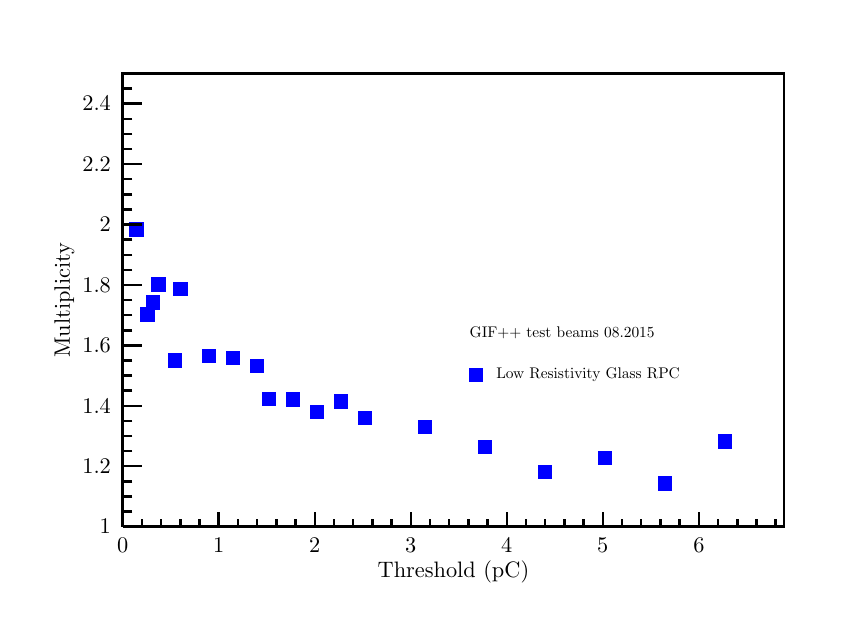
\begin{tikzpicture}
\pgfdeclareplotmark{cross} {
\pgfpathmoveto{\pgfpoint{-0.3\pgfplotmarksize}{\pgfplotmarksize}}
\pgfpathlineto{\pgfpoint{+0.3\pgfplotmarksize}{\pgfplotmarksize}}
\pgfpathlineto{\pgfpoint{+0.3\pgfplotmarksize}{0.3\pgfplotmarksize}}
\pgfpathlineto{\pgfpoint{+1\pgfplotmarksize}{0.3\pgfplotmarksize}}
\pgfpathlineto{\pgfpoint{+1\pgfplotmarksize}{-0.3\pgfplotmarksize}}
\pgfpathlineto{\pgfpoint{+0.3\pgfplotmarksize}{-0.3\pgfplotmarksize}}
\pgfpathlineto{\pgfpoint{+0.3\pgfplotmarksize}{-1.\pgfplotmarksize}}
\pgfpathlineto{\pgfpoint{-0.3\pgfplotmarksize}{-1.\pgfplotmarksize}}
\pgfpathlineto{\pgfpoint{-0.3\pgfplotmarksize}{-0.3\pgfplotmarksize}}
\pgfpathlineto{\pgfpoint{-1.\pgfplotmarksize}{-0.3\pgfplotmarksize}}
\pgfpathlineto{\pgfpoint{-1.\pgfplotmarksize}{0.3\pgfplotmarksize}}
\pgfpathlineto{\pgfpoint{-0.3\pgfplotmarksize}{0.3\pgfplotmarksize}}
\pgfpathclose
\pgfusepathqstroke
}
\pgfdeclareplotmark{cross*} {
\pgfpathmoveto{\pgfpoint{-0.3\pgfplotmarksize}{\pgfplotmarksize}}
\pgfpathlineto{\pgfpoint{+0.3\pgfplotmarksize}{\pgfplotmarksize}}
\pgfpathlineto{\pgfpoint{+0.3\pgfplotmarksize}{0.3\pgfplotmarksize}}
\pgfpathlineto{\pgfpoint{+1\pgfplotmarksize}{0.3\pgfplotmarksize}}
\pgfpathlineto{\pgfpoint{+1\pgfplotmarksize}{-0.3\pgfplotmarksize}}
\pgfpathlineto{\pgfpoint{+0.3\pgfplotmarksize}{-0.3\pgfplotmarksize}}
\pgfpathlineto{\pgfpoint{+0.3\pgfplotmarksize}{-1.\pgfplotmarksize}}
\pgfpathlineto{\pgfpoint{-0.3\pgfplotmarksize}{-1.\pgfplotmarksize}}
\pgfpathlineto{\pgfpoint{-0.3\pgfplotmarksize}{-0.3\pgfplotmarksize}}
\pgfpathlineto{\pgfpoint{-1.\pgfplotmarksize}{-0.3\pgfplotmarksize}}
\pgfpathlineto{\pgfpoint{-1.\pgfplotmarksize}{0.3\pgfplotmarksize}}
\pgfpathlineto{\pgfpoint{-0.3\pgfplotmarksize}{0.3\pgfplotmarksize}}
\pgfpathclose
\pgfusepathqfillstroke
}
\pgfdeclareplotmark{newstar} {
\pgfpathmoveto{\pgfqpoint{0pt}{\pgfplotmarksize}}
\pgfpathlineto{\pgfqpointpolar{44}{0.5\pgfplotmarksize}}
\pgfpathlineto{\pgfqpointpolar{18}{\pgfplotmarksize}}
\pgfpathlineto{\pgfqpointpolar{-20}{0.5\pgfplotmarksize}}
\pgfpathlineto{\pgfqpointpolar{-54}{\pgfplotmarksize}}
\pgfpathlineto{\pgfqpointpolar{-90}{0.5\pgfplotmarksize}}
\pgfpathlineto{\pgfqpointpolar{234}{\pgfplotmarksize}}
\pgfpathlineto{\pgfqpointpolar{198}{0.5\pgfplotmarksize}}
\pgfpathlineto{\pgfqpointpolar{162}{\pgfplotmarksize}}
\pgfpathlineto{\pgfqpointpolar{134}{0.5\pgfplotmarksize}}
\pgfpathclose
\pgfusepathqstroke
}
\pgfdeclareplotmark{newstar*} {
\pgfpathmoveto{\pgfqpoint{0pt}{\pgfplotmarksize}}
\pgfpathlineto{\pgfqpointpolar{44}{0.5\pgfplotmarksize}}
\pgfpathlineto{\pgfqpointpolar{18}{\pgfplotmarksize}}
\pgfpathlineto{\pgfqpointpolar{-20}{0.5\pgfplotmarksize}}
\pgfpathlineto{\pgfqpointpolar{-54}{\pgfplotmarksize}}
\pgfpathlineto{\pgfqpointpolar{-90}{0.5\pgfplotmarksize}}
\pgfpathlineto{\pgfqpointpolar{234}{\pgfplotmarksize}}
\pgfpathlineto{\pgfqpointpolar{198}{0.5\pgfplotmarksize}}
\pgfpathlineto{\pgfqpointpolar{162}{\pgfplotmarksize}}
\pgfpathlineto{\pgfqpointpolar{134}{0.5\pgfplotmarksize}}
\pgfpathclose
\pgfusepathqfillstroke
}
\definecolor{c}{rgb}{1,1,1};
\draw [color=c, fill=c] (0,0) rectangle (10,7.19298);
\definecolor{c}{rgb}{0,0,0};
\draw [c,line width=0.9] (1.2,0.863158) -- (1.2,6.61754) -- (9.6,6.61754) -- (9.6,0.863158) -- (1.2,0.863158);
\draw [c,line width=0.9] (1.2,0.863158) -- (1.2,6.61754) -- (9.6,6.61754) -- (9.6,0.863158) -- (1.2,0.863158);
\draw [c,line width=0.9] (1.2,0.863158) -- (1.2,6.61754) -- (9.6,6.61754) -- (9.6,0.863158) -- (1.2,0.863158);
\draw [c,line width=0.9] (1.2,0.863158) -- (1.2,6.61754) -- (9.6,6.61754) -- (9.6,0.863158) -- (1.2,0.863158);
\draw [c,line width=0.9] (1.2,0.863158) -- (9.6,0.863158);
\draw [c,line width=0.9] (1.2,1.04442) -- (1.2,0.863158);
\draw [c,line width=0.9] (1.44389,0.953789) -- (1.44389,0.863158);
\draw [c,line width=0.9] (1.68779,0.953789) -- (1.68779,0.863158);
\draw [c,line width=0.9] (1.93168,0.953789) -- (1.93168,0.863158);
\draw [c,line width=0.9] (2.17558,0.953789) -- (2.17558,0.863158);
\draw [c,line width=0.9] (2.41947,1.04442) -- (2.41947,0.863158);
\draw [c,line width=0.9] (2.66337,0.953789) -- (2.66337,0.863158);
\draw [c,line width=0.9] (2.90726,0.953789) -- (2.90726,0.863158);
\draw [c,line width=0.9] (3.15116,0.953789) -- (3.15116,0.863158);
\draw [c,line width=0.9] (3.39505,0.953789) -- (3.39505,0.863158);
\draw [c,line width=0.9] (3.63895,1.04442) -- (3.63895,0.863158);
\draw [c,line width=0.9] (3.88284,0.953789) -- (3.88284,0.863158);
\draw [c,line width=0.9] (4.12674,0.953789) -- (4.12674,0.863158);
\draw [c,line width=0.9] (4.37063,0.953789) -- (4.37063,0.863158);
\draw [c,line width=0.9] (4.61453,0.953789) -- (4.61453,0.863158);
\draw [c,line width=0.9] (4.85842,1.04442) -- (4.85842,0.863158);
\draw [c,line width=0.9] (5.10232,0.953789) -- (5.10232,0.863158);
\draw [c,line width=0.9] (5.34621,0.953789) -- (5.34621,0.863158);
\draw [c,line width=0.9] (5.59011,0.953789) -- (5.59011,0.863158);
\draw [c,line width=0.9] (5.834,0.953789) -- (5.834,0.863158);
\draw [c,line width=0.9] (6.0779,1.04442) -- (6.0779,0.863158);
\draw [c,line width=0.9] (6.32179,0.953789) -- (6.32179,0.863158);
\draw [c,line width=0.9] (6.56569,0.953789) -- (6.56569,0.863158);
\draw [c,line width=0.9] (6.80958,0.953789) -- (6.80958,0.863158);
\draw [c,line width=0.9] (7.05348,0.953789) -- (7.05348,0.863158);
\draw [c,line width=0.9] (7.29737,1.04442) -- (7.29737,0.863158);
\draw [c,line width=0.9] (7.54127,0.953789) -- (7.54127,0.863158);
\draw [c,line width=0.9] (7.78516,0.953789) -- (7.78516,0.863158);
\draw [c,line width=0.9] (8.02906,0.953789) -- (8.02906,0.863158);
\draw [c,line width=0.9] (8.27295,0.953789) -- (8.27295,0.863158);
\draw [c,line width=0.9] (8.51685,1.04442) -- (8.51685,0.863158);
\draw [c,line width=0.9] (8.51685,1.04442) -- (8.51685,0.863158);
\draw [c,line width=0.9] (8.76074,0.953789) -- (8.76074,0.863158);
\draw [c,line width=0.9] (9.00464,0.953789) -- (9.00464,0.863158);
\draw [c,line width=0.9] (9.24853,0.953789) -- (9.24853,0.863158);
\draw [c,line width=0.9] (9.49242,0.953789) -- (9.49242,0.863158);
\draw [anchor=base] (1.2,0.539474) node[scale=0.807119, color=c, rotate=0]{0};
\draw [anchor=base] (2.41947,0.539474) node[scale=0.807119, color=c, rotate=0]{1};
\draw [anchor=base] (3.63895,0.539474) node[scale=0.807119, color=c, rotate=0]{2};
\draw [anchor=base] (4.85842,0.539474) node[scale=0.807119, color=c, rotate=0]{3};
\draw [anchor=base] (6.0779,0.539474) node[scale=0.807119, color=c, rotate=0]{4};
\draw [anchor=base] (7.29737,0.539474) node[scale=0.807119, color=c, rotate=0]{5};
\draw [anchor=base] (8.51685,0.539474) node[scale=0.807119, color=c, rotate=0]{6};
\draw (5.4,0.287719) node[scale=0.807119, color=c, rotate=0]{Threshold (pC)};
\draw [c,line width=0.9] (1.2,0.863158) -- (1.2,6.61754);
\draw [c,line width=0.9] (1.44,0.863158) -- (1.2,0.863158);
\draw [c,line width=0.9] (1.32,1.05497) -- (1.2,1.05497);
\draw [c,line width=0.9] (1.32,1.24678) -- (1.2,1.24678);
\draw [c,line width=0.9] (1.32,1.4386) -- (1.2,1.4386);
\draw [c,line width=0.9] (1.44,1.63041) -- (1.2,1.63041);
\draw [c,line width=0.9] (1.32,1.82222) -- (1.2,1.82222);
\draw [c,line width=0.9] (1.32,2.01404) -- (1.2,2.01404);
\draw [c,line width=0.9] (1.32,2.20585) -- (1.2,2.20585);
\draw [c,line width=0.9] (1.44,2.39766) -- (1.2,2.39766);
\draw [c,line width=0.9] (1.32,2.58947) -- (1.2,2.58947);
\draw [c,line width=0.9] (1.32,2.78129) -- (1.2,2.78129);
\draw [c,line width=0.9] (1.32,2.9731) -- (1.2,2.9731);
\draw [c,line width=0.9] (1.44,3.16491) -- (1.2,3.16491);
\draw [c,line width=0.9] (1.32,3.35673) -- (1.2,3.35673);
\draw [c,line width=0.9] (1.32,3.54854) -- (1.2,3.54854);
\draw [c,line width=0.9] (1.32,3.74035) -- (1.2,3.74035);
\draw [c,line width=0.9] (1.44,3.93216) -- (1.2,3.93216);
\draw [c,line width=0.9] (1.32,4.12398) -- (1.2,4.12398);
\draw [c,line width=0.9] (1.32,4.31579) -- (1.2,4.31579);
\draw [c,line width=0.9] (1.32,4.5076) -- (1.2,4.5076);
\draw [c,line width=0.9] (1.44,4.69942) -- (1.2,4.69942);
\draw [c,line width=0.9] (1.32,4.89123) -- (1.2,4.89123);
\draw [c,line width=0.9] (1.32,5.08304) -- (1.2,5.08304);
\draw [c,line width=0.9] (1.32,5.27485) -- (1.2,5.27485);
\draw [c,line width=0.9] (1.44,5.46667) -- (1.2,5.46667);
\draw [c,line width=0.9] (1.32,5.65848) -- (1.2,5.65848);
\draw [c,line width=0.9] (1.32,5.85029) -- (1.2,5.85029);
\draw [c,line width=0.9] (1.32,6.04211) -- (1.2,6.04211);
\draw [c,line width=0.9] (1.44,6.23392) -- (1.2,6.23392);
\draw [c,line width=0.9] (1.44,6.23392) -- (1.2,6.23392);
\draw [c,line width=0.9] (1.32,6.42573) -- (1.2,6.42573);
\draw [c,line width=0.9] (1.32,6.61754) -- (1.2,6.61754);
\draw [anchor= east] (1.15,0.863158) node[scale=0.807119, color=c, rotate=0]{1};
\draw [anchor= east] (1.15,1.63041) node[scale=0.807119, color=c, rotate=0]{1.2};
\draw [anchor= east] (1.15,2.39766) node[scale=0.807119, color=c, rotate=0]{1.4};
\draw [anchor= east] (1.15,3.16491) node[scale=0.807119, color=c, rotate=0]{1.6};
\draw [anchor= east] (1.15,3.93216) node[scale=0.807119, color=c, rotate=0]{1.8};
\draw [anchor= east] (1.15,4.69942) node[scale=0.807119, color=c, rotate=0]{2};
\draw [anchor= east] (1.15,5.46667) node[scale=0.807119, color=c, rotate=0]{2.2};
\draw [anchor= east] (1.15,6.23392) node[scale=0.807119, color=c, rotate=0]{2.4};
\draw (0.458145,3.74035) node[scale=0.807119, color=c, rotate=90]{Multiplicity};
\definecolor{c}{rgb}{0,0,1};
\foreach \P in {(1.37421,4.63547), (1.51358,3.55767), (1.58326,3.71112), (1.65295,3.9406), (1.862,2.97137), (1.93168,3.88187), (1.93168,3.88187), (2.29753,3.03149), (2.6024,3.00141), (2.90726,2.90623), (3.0597,2.48735), (3.36457,2.47538),
 (3.66944,2.31925), (3.9743,2.45455), (4.27917,2.23961), (5.04134,2.13054), (5.80352,1.87601), (6.56569,1.55718), (7.32786,1.73759), (8.09003,1.41328), (8.8522,1.94211)}{\draw[mark options={color=c,fill=c},mark size=2.402402pt,mark=square*] plot
 coordinates {\P};}
\definecolor{c}{rgb}{1,1,1};
\draw [color=c, fill=c] (5.5,2.51754) rectangle (7,3.59649);
\definecolor{c}{rgb}{0,0,0};
\draw [anchor= west] (5.5375,3.32675) node[scale=0.556634, color=c, rotate=0]{GIF++ test beams 08.2015};
\draw [anchor= west] (5.875,2.78728) node[scale=0.556634, color=c, rotate=0]{Low Resistivity Glass RPC};
\definecolor{c}{rgb}{0,0,1};
\foreach \P in {(5.6875,2.78728)}{\draw[mark options={color=c,fill=c},mark size=2.402402pt,mark=square*] plot coordinates {\P};}
\definecolor{c}{rgb}{0,0,0};
\draw [c,line width=0.9] (1.2,0.863158) -- (9.6,0.863158);
\draw [c,line width=0.9] (1.2,1.04442) -- (1.2,0.863158);
\draw [c,line width=0.9] (1.44389,0.953789) -- (1.44389,0.863158);
\draw [c,line width=0.9] (1.68779,0.953789) -- (1.68779,0.863158);
\draw [c,line width=0.9] (1.93168,0.953789) -- (1.93168,0.863158);
\draw [c,line width=0.9] (2.17558,0.953789) -- (2.17558,0.863158);
\draw [c,line width=0.9] (2.41947,1.04442) -- (2.41947,0.863158);
\draw [c,line width=0.9] (2.66337,0.953789) -- (2.66337,0.863158);
\draw [c,line width=0.9] (2.90726,0.953789) -- (2.90726,0.863158);
\draw [c,line width=0.9] (3.15116,0.953789) -- (3.15116,0.863158);
\draw [c,line width=0.9] (3.39505,0.953789) -- (3.39505,0.863158);
\draw [c,line width=0.9] (3.63895,1.04442) -- (3.63895,0.863158);
\draw [c,line width=0.9] (3.88284,0.953789) -- (3.88284,0.863158);
\draw [c,line width=0.9] (4.12674,0.953789) -- (4.12674,0.863158);
\draw [c,line width=0.9] (4.37063,0.953789) -- (4.37063,0.863158);
\draw [c,line width=0.9] (4.61453,0.953789) -- (4.61453,0.863158);
\draw [c,line width=0.9] (4.85842,1.04442) -- (4.85842,0.863158);
\draw [c,line width=0.9] (5.10232,0.953789) -- (5.10232,0.863158);
\draw [c,line width=0.9] (5.34621,0.953789) -- (5.34621,0.863158);
\draw [c,line width=0.9] (5.59011,0.953789) -- (5.59011,0.863158);
\draw [c,line width=0.9] (5.834,0.953789) -- (5.834,0.863158);
\draw [c,line width=0.9] (6.0779,1.04442) -- (6.0779,0.863158);
\draw [c,line width=0.9] (6.32179,0.953789) -- (6.32179,0.863158);
\draw [c,line width=0.9] (6.56569,0.953789) -- (6.56569,0.863158);
\draw [c,line width=0.9] (6.80958,0.953789) -- (6.80958,0.863158);
\draw [c,line width=0.9] (7.05348,0.953789) -- (7.05348,0.863158);
\draw [c,line width=0.9] (7.29737,1.04442) -- (7.29737,0.863158);
\draw [c,line width=0.9] (7.54127,0.953789) -- (7.54127,0.863158);
\draw [c,line width=0.9] (7.78516,0.953789) -- (7.78516,0.863158);
\draw [c,line width=0.9] (8.02906,0.953789) -- (8.02906,0.863158);
\draw [c,line width=0.9] (8.27295,0.953789) -- (8.27295,0.863158);
\draw [c,line width=0.9] (8.51685,1.04442) -- (8.51685,0.863158);
\draw [c,line width=0.9] (8.51685,1.04442) -- (8.51685,0.863158);
\draw [c,line width=0.9] (8.76074,0.953789) -- (8.76074,0.863158);
\draw [c,line width=0.9] (9.00464,0.953789) -- (9.00464,0.863158);
\draw [c,line width=0.9] (9.24853,0.953789) -- (9.24853,0.863158);
\draw [c,line width=0.9] (9.49242,0.953789) -- (9.49242,0.863158);
\draw [c,line width=0.9] (1.2,0.863158) -- (1.2,6.61754);
\draw [c,line width=0.9] (1.44,0.863158) -- (1.2,0.863158);
\draw [c,line width=0.9] (1.32,1.05497) -- (1.2,1.05497);
\draw [c,line width=0.9] (1.32,1.24678) -- (1.2,1.24678);
\draw [c,line width=0.9] (1.32,1.4386) -- (1.2,1.4386);
\draw [c,line width=0.9] (1.44,1.63041) -- (1.2,1.63041);
\draw [c,line width=0.9] (1.32,1.82222) -- (1.2,1.82222);
\draw [c,line width=0.9] (1.32,2.01404) -- (1.2,2.01404);
\draw [c,line width=0.9] (1.32,2.20585) -- (1.2,2.20585);
\draw [c,line width=0.9] (1.44,2.39766) -- (1.2,2.39766);
\draw [c,line width=0.9] (1.32,2.58947) -- (1.2,2.58947);
\draw [c,line width=0.9] (1.32,2.78129) -- (1.2,2.78129);
\draw [c,line width=0.9] (1.32,2.9731) -- (1.2,2.9731);
\draw [c,line width=0.9] (1.44,3.16491) -- (1.2,3.16491);
\draw [c,line width=0.9] (1.32,3.35673) -- (1.2,3.35673);
\draw [c,line width=0.9] (1.32,3.54854) -- (1.2,3.54854);
\draw [c,line width=0.9] (1.32,3.74035) -- (1.2,3.74035);
\draw [c,line width=0.9] (1.44,3.93216) -- (1.2,3.93216);
\draw [c,line width=0.9] (1.32,4.12398) -- (1.2,4.12398);
\draw [c,line width=0.9] (1.32,4.31579) -- (1.2,4.31579);
\draw [c,line width=0.9] (1.32,4.5076) -- (1.2,4.5076);
\draw [c,line width=0.9] (1.44,4.69942) -- (1.2,4.69942);
\draw [c,line width=0.9] (1.32,4.89123) -- (1.2,4.89123);
\draw [c,line width=0.9] (1.32,5.08304) -- (1.2,5.08304);
\draw [c,line width=0.9] (1.32,5.27485) -- (1.2,5.27485);
\draw [c,line width=0.9] (1.44,5.46667) -- (1.2,5.46667);
\draw [c,line width=0.9] (1.32,5.65848) -- (1.2,5.65848);
\draw [c,line width=0.9] (1.32,5.85029) -- (1.2,5.85029);
\draw [c,line width=0.9] (1.32,6.04211) -- (1.2,6.04211);
\draw [c,line width=0.9] (1.44,6.23392) -- (1.2,6.23392);
\draw [c,line width=0.9] (1.44,6.23392) -- (1.2,6.23392);
\draw [c,line width=0.9] (1.32,6.42573) -- (1.2,6.42573);
\draw [c,line width=0.9] (1.32,6.61754) -- (1.2,6.61754);
\draw [c,line width=0.9] (1.2,0.863158) -- (1.2,6.61754) -- (9.6,6.61754) -- (9.6,0.863158) -- (1.2,0.863158);
\draw [c,line width=0.9] (1.2,0.863158) -- (1.2,6.61754) -- (9.6,6.61754) -- (9.6,0.863158) -- (1.2,0.863158);
\end{tikzpicture}
